\documentclass[12pt]{article}
\usepackage{amsfonts, amssymb, amsmath, amsthm}
\usepackage[margin=1in]{geometry}
\usepackage{tikz}

\title{Explainer: Problem 1 (Rudin 7.6) --- Alternating Series of Functions}
\author{}
\date{}

\begin{document}
\maketitle

\section*{What's going on?}
We have the series $\sum_{n=1}^{\infty} (-1)^n \frac{x^2 + n}{n^2}$. The signs alternate ($+, -, +, -, \ldots$), and the terms depend on $x$. We need to show two things:
\begin{enumerate}
    \item On any bounded interval $[-M, M]$, the series converges \textbf{uniformly}.
    \item For every single $x$, the series does \textbf{not} converge absolutely.
\end{enumerate}

\section*{Key definitions}

\textbf{Uniform convergence of a series:} $\sum f_n$ converges uniformly on $E$ if the partial sums $S_N(x) = \sum_{n=1}^N f_n(x)$ converge uniformly, i.e.\ $\sup_{x \in E} |S(x) - S_N(x)| \to 0$.

\textbf{Absolute convergence:} $\sum f_n(x)$ converges absolutely at $x$ if $\sum |f_n(x)| < \infty$.

\section*{Splitting the series}

The key idea: split the $n$th term into two pieces:
$$
(-1)^n \frac{x^2 + n}{n^2} = (-1)^n \frac{x^2}{n^2} + (-1)^n \frac{1}{n}.
$$

\begin{center}
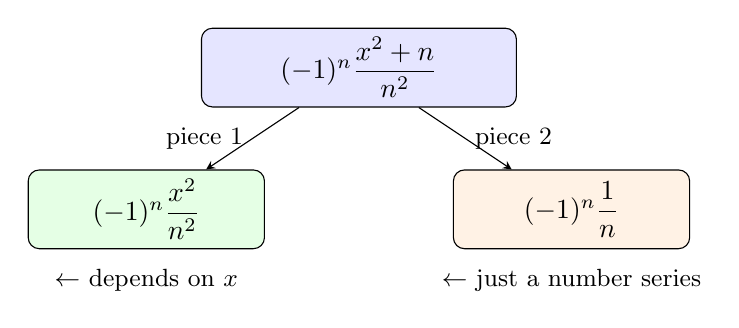
\begin{tikzpicture}[>=stealth, scale=0.9]
    \node[draw, rounded corners, fill=blue!10, minimum width=4cm, minimum height=1cm] (orig) at (0,2) {$(-1)^n \dfrac{x^2+n}{n^2}$};
    \node[draw, rounded corners, fill=green!10, minimum width=3cm, minimum height=1cm] (A) at (-3,0) {$(-1)^n \dfrac{x^2}{n^2}$};
    \node[draw, rounded corners, fill=orange!10, minimum width=3cm, minimum height=1cm] (B) at (3,0) {$(-1)^n \dfrac{1}{n}$};
    \draw[->] (orig) -- (A) node[midway, left] {\small piece 1};
    \draw[->] (orig) -- (B) node[midway, right] {\small piece 2};
    \node[below] at (-3,-0.7) {\small $\leftarrow$ depends on $x$};
    \node[below] at (3,-0.7) {\small $\leftarrow$ just a number series};
\end{tikzpicture}
\end{center}

\section*{Strategy for uniform convergence}

\textbf{Piece 2} ($\sum (-1)^n / n$): This is just the alternating harmonic series --- a fixed number, no $x$-dependence. It converges (to $-\ln 2$). A constant partial sum trivially converges uniformly.

\textbf{Piece 1} ($\sum (-1)^n x^2/n^2$): Factor out $x^2$ to get $x^2 \sum (-1)^n/n^2$. On a bounded interval $|x| \leq M$, you can bound $|x^2/n^2| \leq M^2/n^2$. Since $\sum M^2/n^2 < \infty$, the \textbf{Weierstrass $M$-test} gives uniform (and absolute!) convergence.

Combining: a uniformly convergent series plus a (trivially) uniformly convergent constant gives uniform convergence.

\section*{Strategy for no absolute convergence}

Look at $\left|(-1)^n \frac{x^2+n}{n^2}\right| = \frac{x^2+n}{n^2} = \frac{x^2}{n^2} + \frac{1}{n}$.

The $x^2/n^2$ part sums to something finite, but $\sum 1/n = \infty$ (harmonic series!). So $\sum |f_n(x)| = \infty$ for every $x$. The absolute series always diverges.

\section*{Takeaway}

This is a nice example showing that a series can converge uniformly (thanks to cancellation from alternating signs) without converging absolutely. The alternating signs are doing real work here --- they make $\sum (-1)^n/n$ converge even though $\sum 1/n$ doesn't.

\end{document}